\subsubsection{Procedure}\label{procedureGestione}
\subsubsubsection{Apertura di un ticket}
La procedura di apertura di un ticket segue il diagramma di attività riportato in \customRef{fig:aperturaTicket}{figura}, e la sua applicazione è delegata al \rRP, che:
\begin{enumerate}
\item Seleziona la tipologia: \emph{task}, \emph{feature}, \emph{\gloxy{bug}} o \emph{step};
\item Seleziona la categoria specifica: \emph{documentazione} o \emph{verifica};
\item Definisce l'\emph{oggetto};
\item Definisce una \emph{descrizione};
\item Imposta lo \emph{stato} a ``\emph{New}'';
\item Seleziona il livello di \emph{priorità}: \emph{low}, \emph{normal}, \emph{high}, \emph{urgent} o \emph{immediate};
\item Indica una \emph{stima del tempo} (in ore) necessario per portarlo a termine;
\item Definisce una \emph{lista di attività} da compiere (facoltativo);
\item Stabilisce l'\emph{attività principale} da eseguire (facoltativo);
\item Definisce la data di \emph{inizio} (facoltativo);
\item Definisce la data di \emph{scadenza} (facoltativo);
\item Sceglie l'\emph{assegnatario} (facoltativo);
\item Indica degli \emph{osservatori} (facoltativo).
\end{enumerate}
L'assegnatario e gli osservatori del ticket ricevono una notifica via mail che li informa della sua apertura.
\\\textbf{N.B.:} qualora non venga scelto alcun assegnatario, dovrà essere indicato almeno un osservatore.
\begin{figure}[H]
\centering
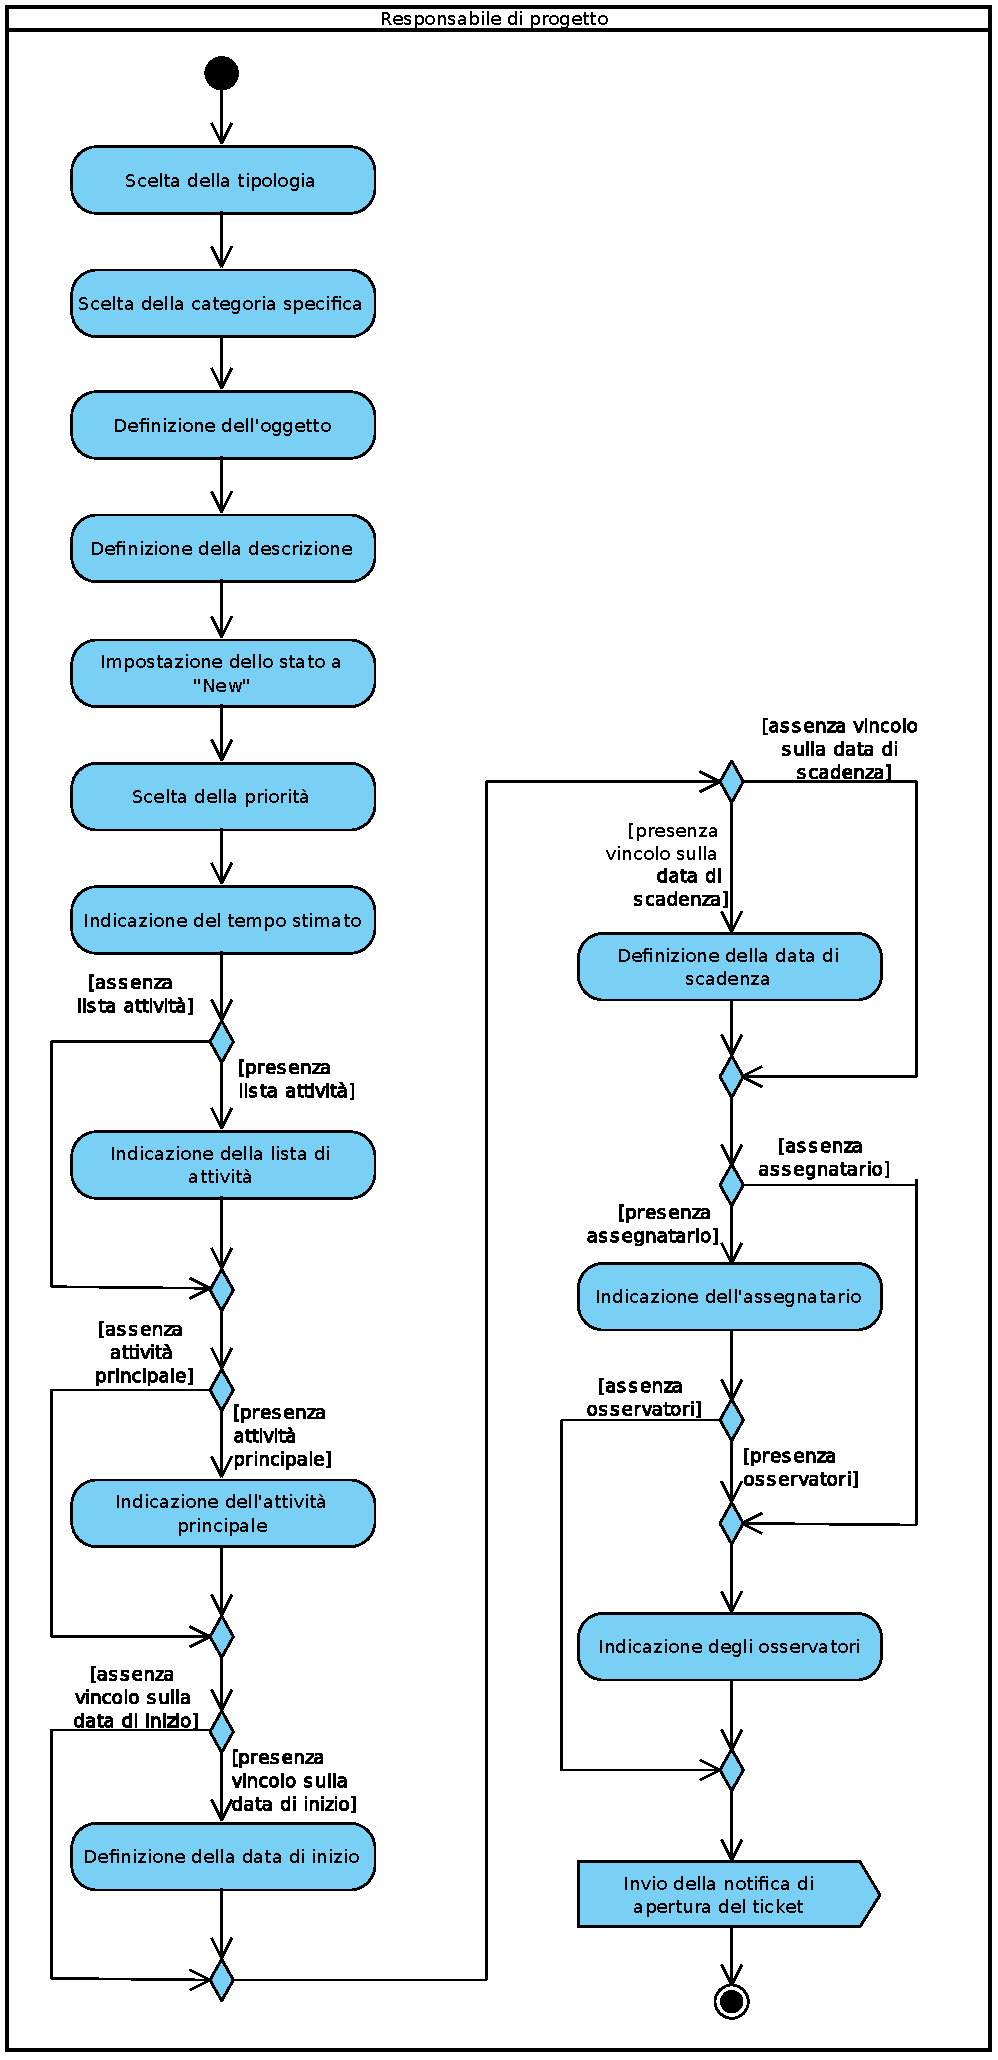
\includegraphics[width=10cm]{../immagini/aperturaTicket.pdf}
\caption{Diagramma di attività - apertura di un ticket}
\label{fig:aperturaTicket}
\end{figure}
\subsubsubsection{Rigetto di un ticket}
La procedura di rigetto di un ticket da parte del \rRP segue il diagramma di attività riportato in \customRef{fig:rigetto_chiusuraTicket}{figura}.
Il \rRP:
\begin{enumerate}
\item Riceve la notifica di un ticket con stato ``Approved'';
\item Effettua una rapida ricerca per trovare eventuali anomalie non catturate dal \rV, che dà esito positivo;
\item Crea una lista con le anomalie trovate;
\item Imposta lo stato del ticket a ``Rejected'' e lo commenta con il link alla lista delle anomalie;
\item Apre i ticket per la correzione delle anomalie;
\item Apre un ticket per la verifica della correzione delle anomalie.
\end{enumerate}
\subsubsubsection{Chiusura di ticket}
La procedura di chiusura di ticket segue il diagramma di attività riportato in \customRef{fig:rigetto_chiusuraTicket}{figura}.
L'attività di chiusura di ticket è delegata al \rRP, che:
\begin{enumerate}
\item Riceve la notifica di un ticket con stato ``Approved'';
\item Effettua una rapida ricerca per trovare eventuali anomalie non catturate dal \rV, che dà esito negativo.
\end{enumerate}
oppure:
\begin{enumerate}
\item Riceve la notifica di un ticket con stato ``Rejected'', accompagnata dalla lista delle anomalie trovate dal verificatore;
\item Apre i ticket per la correzione delle anomalie;
\item Apre un ticket per la verifica della correzione delle anomalie.
\end{enumerate}
Infine, il \rRP imposta lo stato del ticket a ``Closed''.
\begin{figure}[H]
\centering
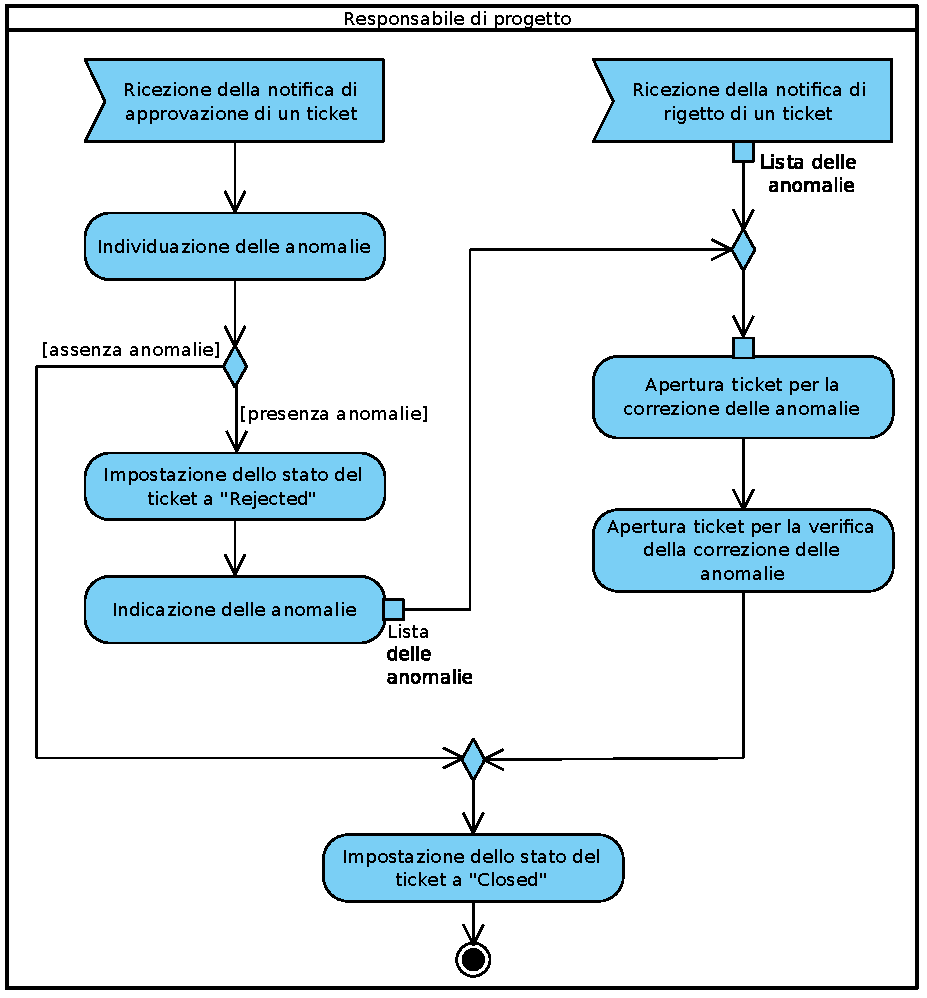
\includegraphics[width=9cm]{../immagini/rigetto_chiusuraTicket.pdf}
\caption{Diagramma di attività - rigetto/chiusura di ticket}
\label{fig:rigetto_chiusuraTicket}
\end{figure}
\subsubsubsection{Rilevazione dei rischi}\label{procRilevazRischi}
In ciascuna fase del \gloxy{progetto}, il \rRP avrà il compito di individuare i rischi indicati nel \PP.
Nel caso si verifichino problematiche non previste, il \rRP dovrà includerle nell’analisi dei rischi.
Complessivamente la procedura di rilevazione dei rischi prevede i seguenti passi:
\begin{enumerate}
\item Rilevazione dei problemi non calcolati;
\item Analisi e classificazione dei nuovi rischi individuati;
\item Pianificazione di controllo dei nuovi rischi individuati;
\item Definizione di contromisure per i nuovi rischi individuati.
\end{enumerate}
\begin{figure}[H]
\centering
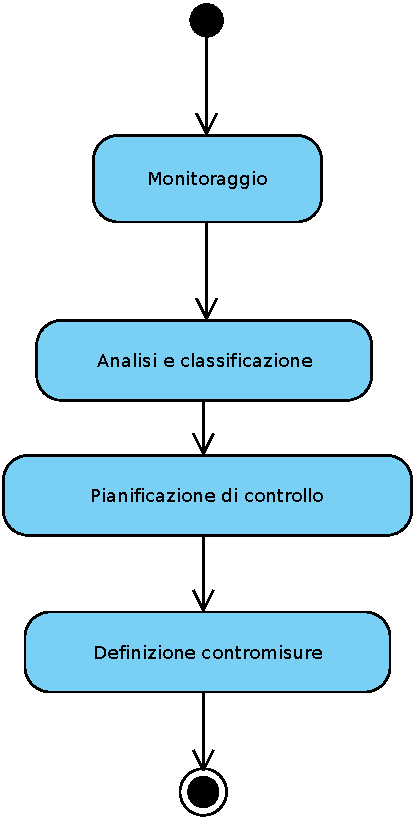
\includegraphics[width=5cm]{../immagini/analisiRischi.pdf}
\caption{Diagramma di attività - rilevazione dei rischi}
\label{fig:rilevazione rischi}
\end{figure}
